\begin{figure}[ht]
%{0.45\textwidth}
  \centering
  \resizebox{.8\linewidth}{!}{
%\begin{adjustbox}{max size={.9\textwidth}}
    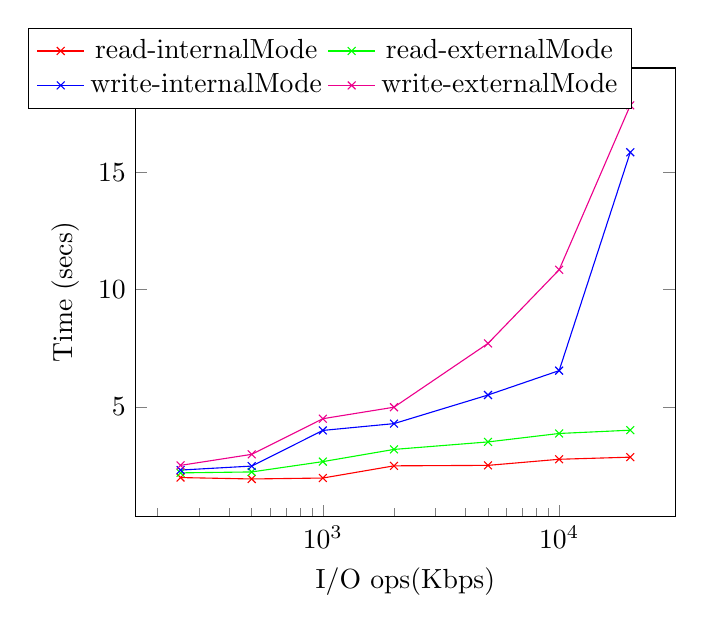
\begin{tikzpicture}
      \begin{axis}[
        xmode=log,
        legend style={at={(-0.2,1.09)},anchor=north west,legend columns=2},
        xlabel=I/O ops(Kbps),
        ylabel=Time (secs)]
        \addplot[color=red,mark=x] coordinates {
          (0,1.85)
          (250,1.99)
          (500,1.93)
          (1000,1.97)
          (2000,2.49)
          (5000,2.51)
          (10000,2.77)
          (20000,2.86)
        };
        \addlegendentry{read-internalMode}
        \addplot[color=green,mark=x] coordinates {
          (0,1.97)
          (250,2.19)
          (500,2.23)
          (1000,2.67)
          (2000,3.19)
          (5000,3.51)
          (10000,3.87)
          (20000,4.01)
        };
        \addlegendentry{read-externalMode}				
        \addplot[color=blue,mark=x] coordinates {
          (0,1.85)
          (250,2.31)
          (500,2.48)
          (1000,4.00)
          (2000,4.29)
          (5000,5.51)
          (10000,6.55)
          (20000,15.86)
        };
        \addlegendentry{write-internalMode}				
        \addplot[color=magenta,mark=x] coordinates {
          (0,1.87)
          (250,2.51)
          (500,2.98)
          (1000,4.50)
          (2000,4.99)
          (5000,7.71)
          (10000,10.85)
          (20000,17.86)
        };
        \addlegendentry{write-externalMode}
      \end{axis}
    \end{tikzpicture}
 % \end{adjustbox}
  }
  %\captionsetup{justification=centering}
  \caption{Live Cloning suspend time with increasing amounts of I/O operations }
  \label{fig:fioResults}
\end{figure}



\subsubsection{Micro Benchmark using I/O operations:}
The main factor that impacts suspend time is the number of ``dirty pages'' in the suspend phase, which have not been copied over in the pre-copy rsync operation (see section~\ref{sec:CloneManager}).
To understand this better, we use \fio (flexible I/O tool for Linux)~\cite{fio}, to gradually increase the number of I/O operations while doing live cloning.
We run the \fio tool to do read and writes of random values with a controlled I/O bandwidth. 
%The suspend time is observed by instrumentation within the cloning script, which reports time taken by each of the suspend processes.
Additionally, we ensure that the I/O job being processed by \fio is long enough to last through the cloning process.

As shown in figure~\ref{fig:fioResults}, read operations have a much smaller impact on suspend time of live cloning compared to write operations.
This can be attributed to the increase of ``dirty pages'' in write operations, whereas for read, the disk image remains largely the same.
The internal mode is much faster than the external mode, as both the production and debug-container are hosted in the same physical device.
We believe, that for higher I/O operations, with a large amount of ``dirty-pages'', network bandwidth becomes a bottleneck: leading to longer suspend times.
Overall in our experiments, the internal mode is able to manage write operation up to 10 Mbps, with a total suspend-time of approx 5 seconds.
Whereas, the external mode is only able to manage up to 5-6 Mbps, for a 5 sec suspend time.\\ \\
